\documentclass[latex/main.tex]{subfiles}

\begin{document}
\section{Results}

\begin{figure}[H]
    \centering
    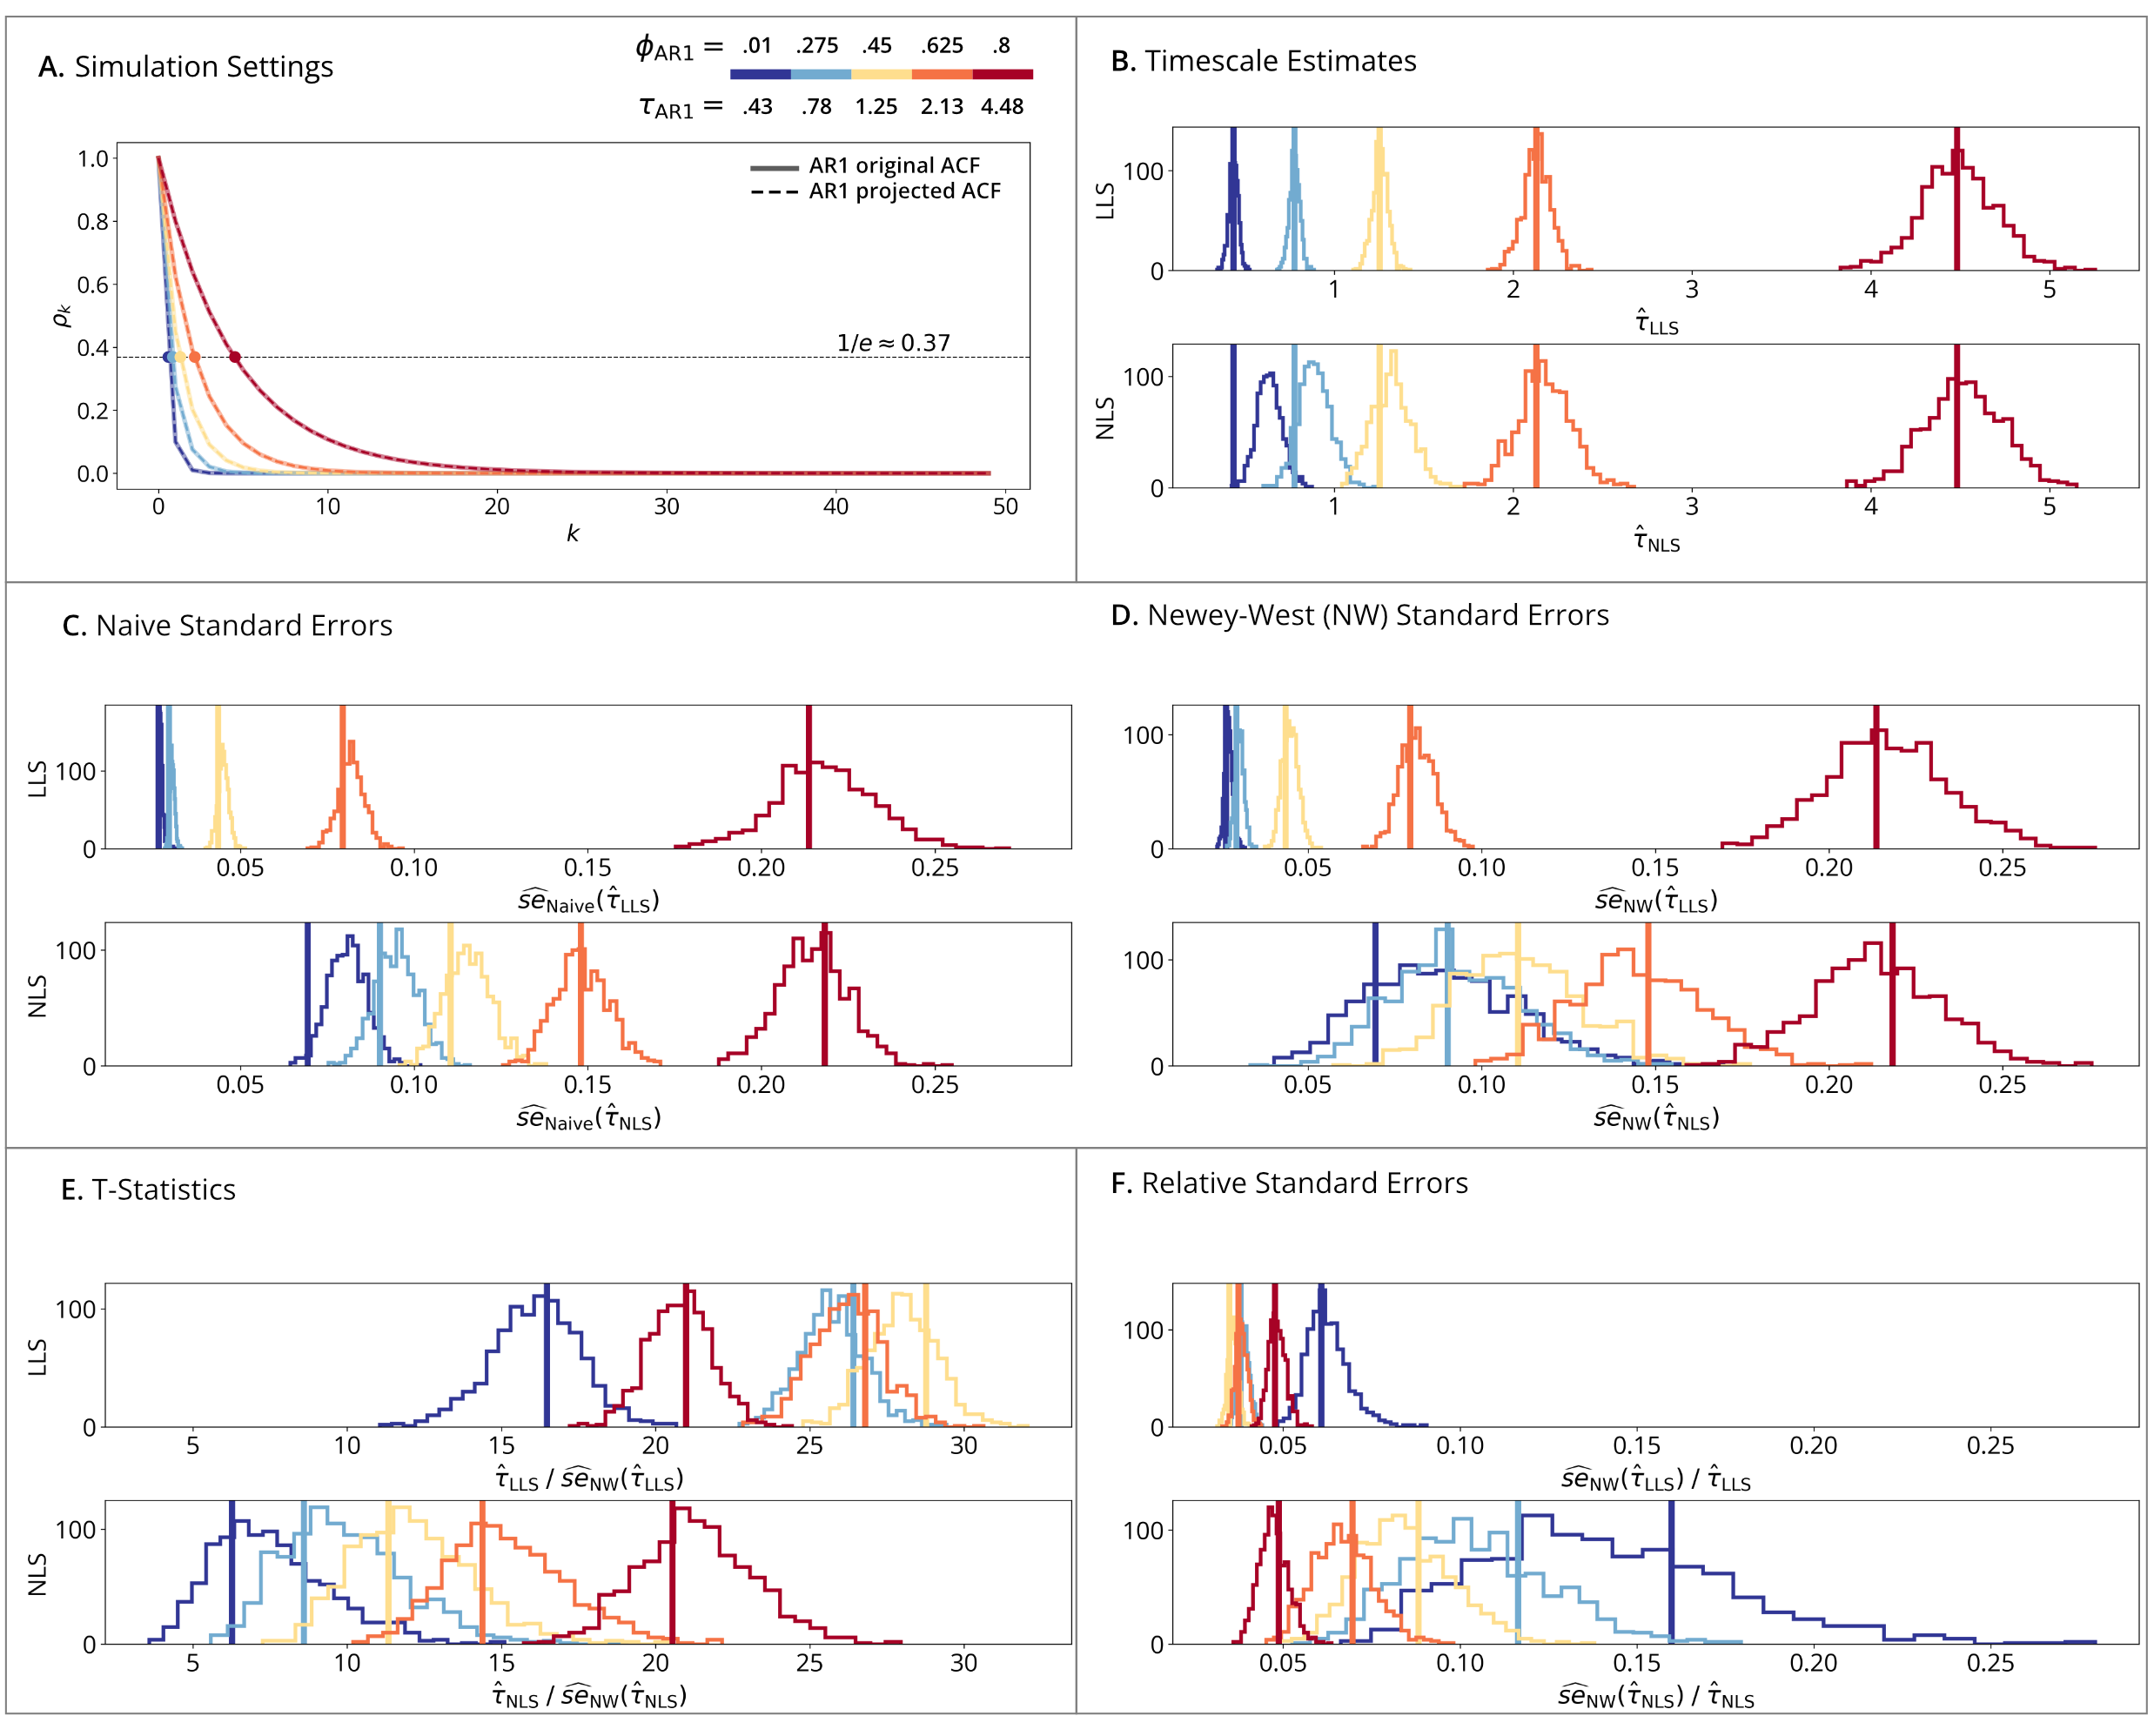
\includegraphics[width=1\textwidth]{latex/results/fig01-ar1.png} 
    \caption{
    \textbf{AR1 simulations}.
    (\textbf{A}) Simulation Settings. Five fixed settings are illustrated, where the solid line represents the original autocorrelation function (ACF), and the dashed line represents the AR1-projected ACF. Since both ACFs follow AR1, they overlap. Solid dots mark the timescale at which the AR1-projected ACF reaches $1/e \approx 0.37$.
    (\textbf{B}) Timescale Estimates. Vertical lines show the true timescale parameters, and histograms show the distribution of timescale estimates across $N=1000$ independent replications. The top plot shows the results for the linear least squares estimator (see \nameref{sec:time-domain-linear-model}), and the bottom plot for the nonlinear least squares estimator (see \nameref{sec:autocorrelation-domain-nonlinear-model}).
    (\textbf{C}) Naive Standard Errors and (\textbf{D}) Newey-West Standard Errors. Vertical lines show the standard deviations of the sampling distributions from panel B, while histograms show the distribution of standard error estimates, using the naive and Newey-West estimators, respectively.
    (\textbf{E}) T-Statistics and (\textbf{F}) Relative Standard Errors. Vertical lines show true values, and histograms show the distributions of the estimates.
    }
    \label{fig:sim-ar1}
\end{figure}

\begin{figure}[H]
    \centering
    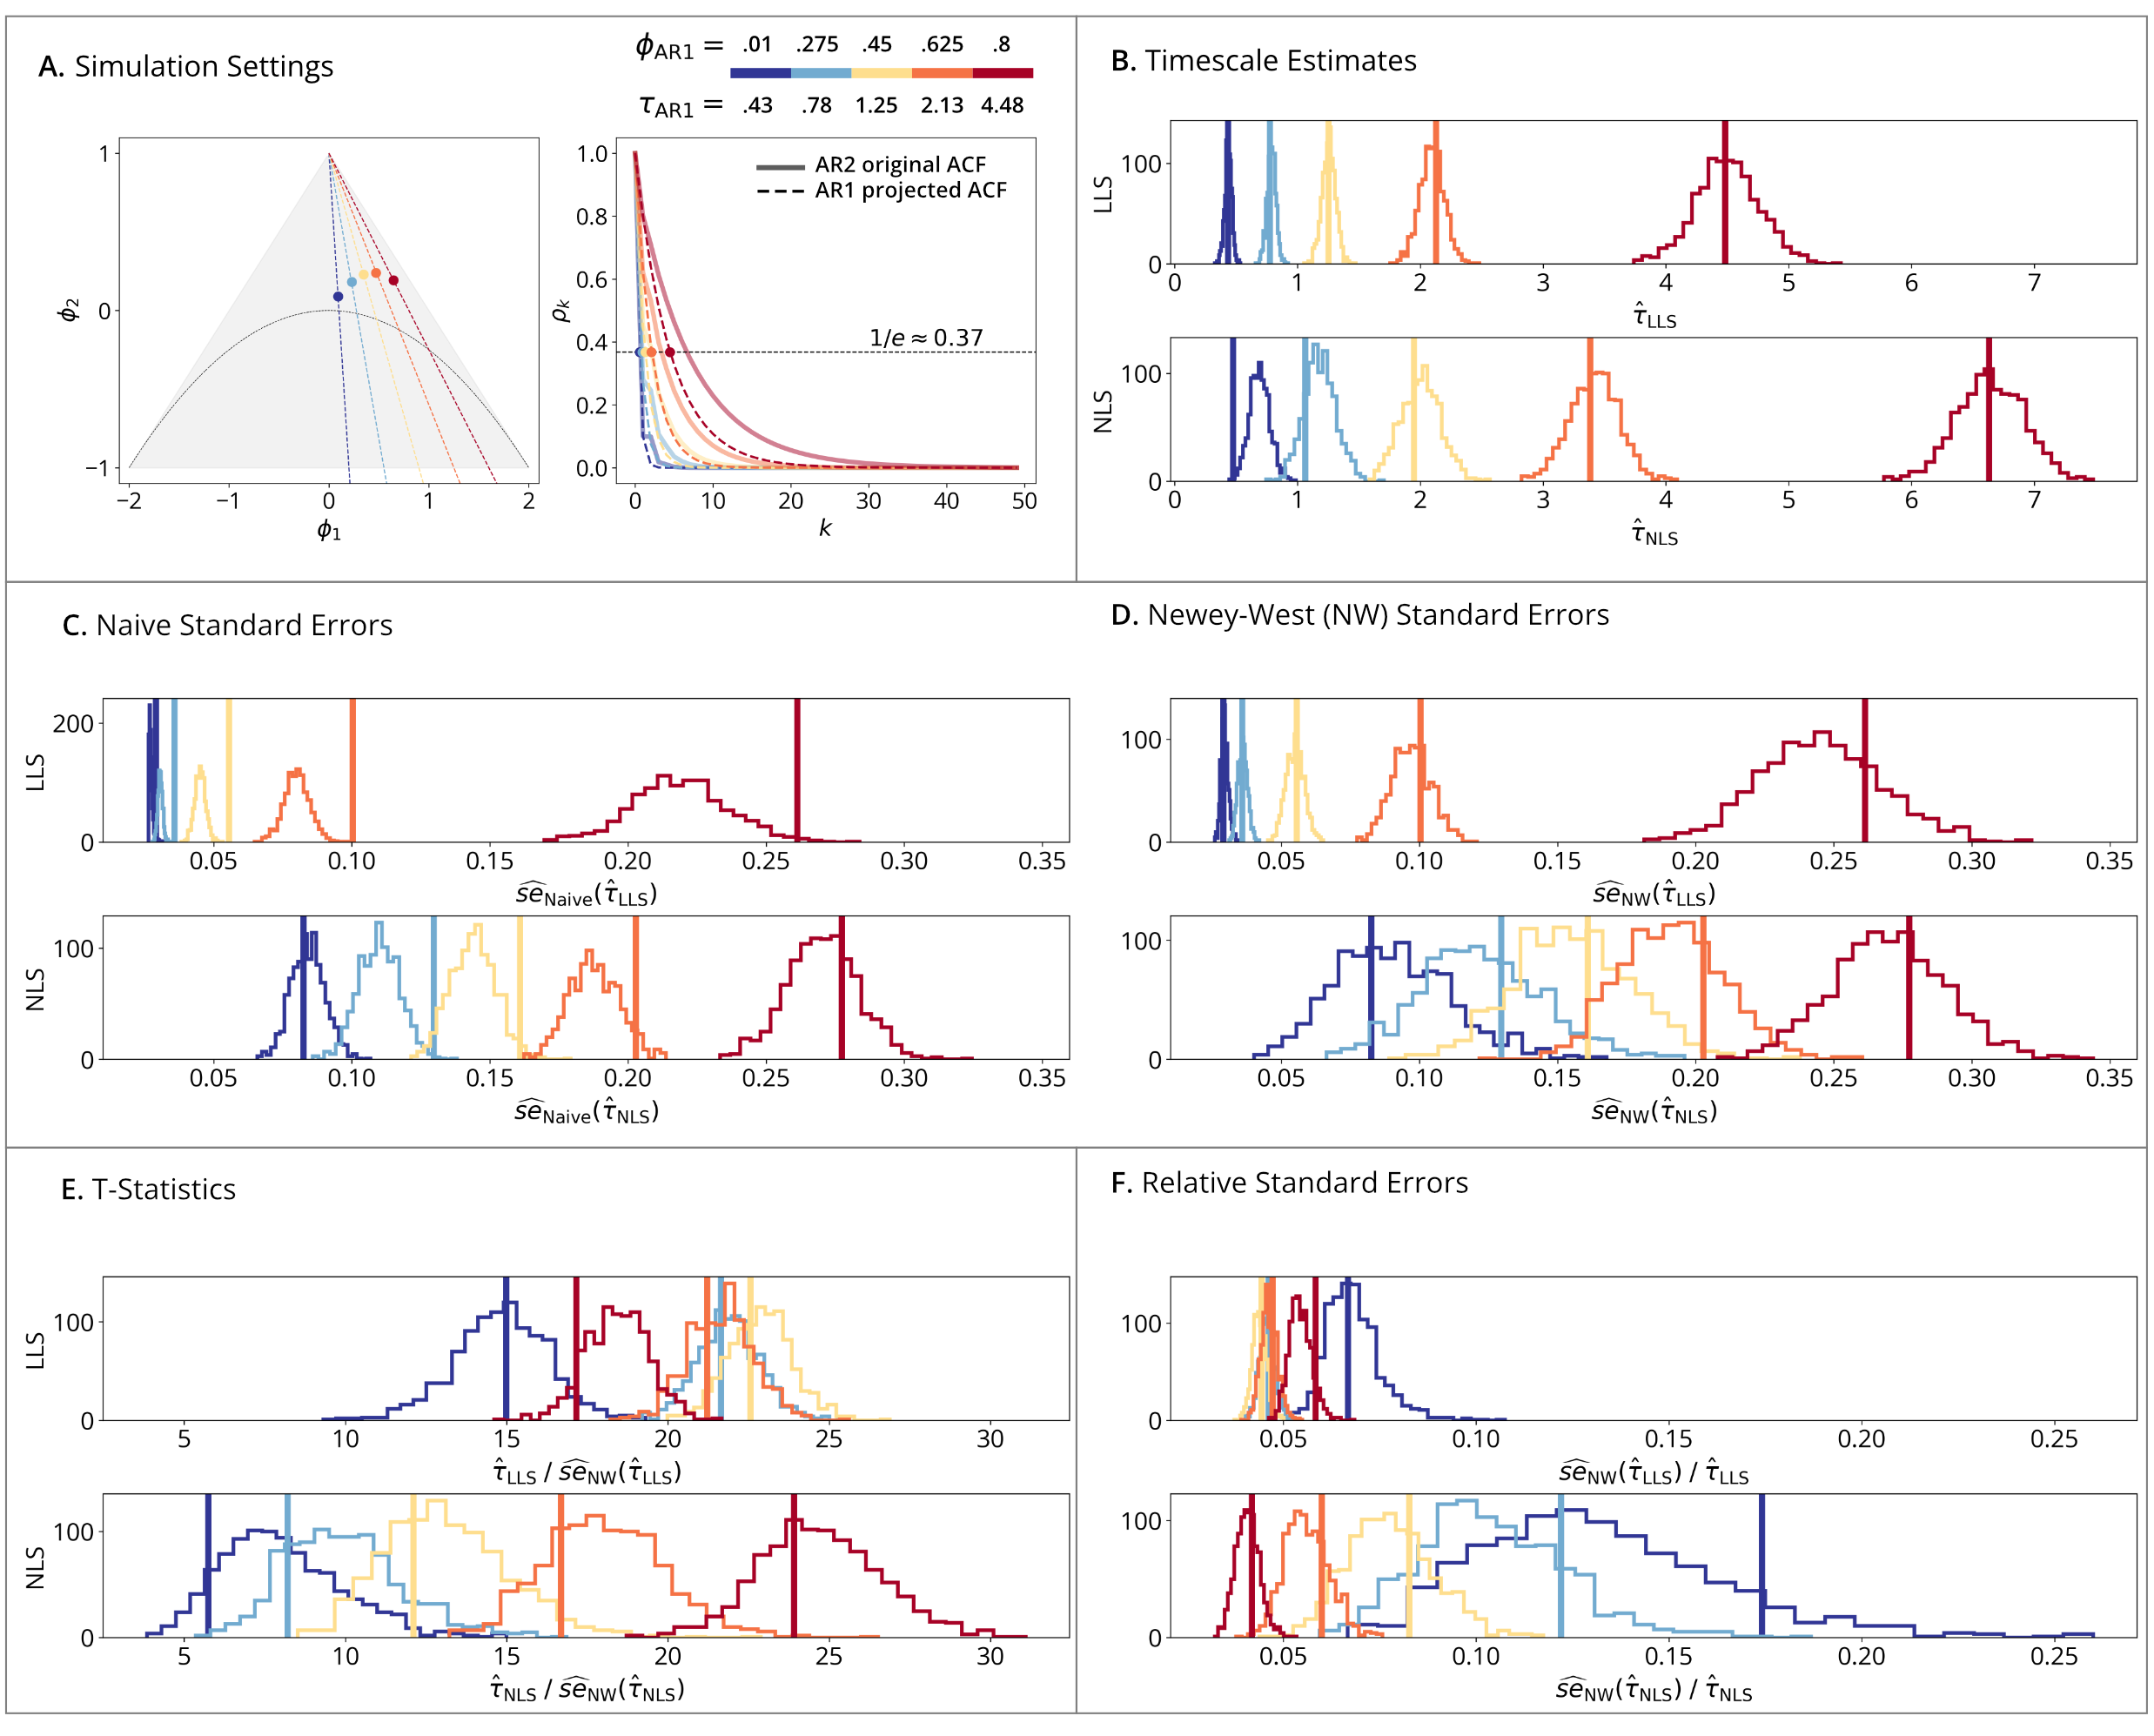
\includegraphics[width=1\textwidth]{latex/results/fig02-ar2.png} 
    \caption{
    \textbf{AR2 simulations}.
    (\textbf{A}) Simulation Settings. The AR2 stationary region (gray triangle) in the $(\phi_1, \phi_2)$ plane is defined by the conditions $\phi_2<1+\phi_1, \phi_2<1-\phi_1, \phi_2>-1$. Within this region, the theoretical boundary between periodic and aperiodic behavior is given by $\phi_2 = -\phi_1^2/4$. Five fixed $(\phi_1, \phi_2)$ pairs within the stationary and aperiodic region were used to simulate AR2 processes with AR1 projections (dashed lines) equivalent to Figure \ref{fig:sim-ar1}. In the autocorrelation domain, the solid lines represents the original autocorrelation function (ACF), and the dashed line represents the AR1-projected ACF. Since the original ACF is AR2 and the projected is AR1, the lines do not overlap. Solid dots mark the timescale at which the AR1-projected ACF reaches $1/e \approx 0.37$.
    (\textbf{B}) Timescale Estimates. Vertical lines show the true timescale parameters, and histograms show the distribution of timescale estimates across $N=1000$ independent replications. The top plot shows the results for the linear least squares estimator (see \nameref{sec:time-domain-linear-model}), and the bottom plot for the nonlinear least squares estimator (see \nameref{sec:autocorrelation-domain-nonlinear-model}). The true values of the two estimators differ because of their respective definitions.
    (\textbf{C}) Naive Standard Errors and (\textbf{D}) Newey-West Standard Errors. Vertical lines show the standard deviations of the sampling distributions from panel B, while histograms show the distribution of standard error estimates, using the naive and Newey-West estimators, respectively.
    (\textbf{E}) T-Statistics and (\textbf{F}) Relative Standard Errors. Vertical lines show true values, and histograms show the distributions of the estimates.
    }
    \label{fig:sim-ar2}
\end{figure}

\begin{figure}[H]
    \centering
    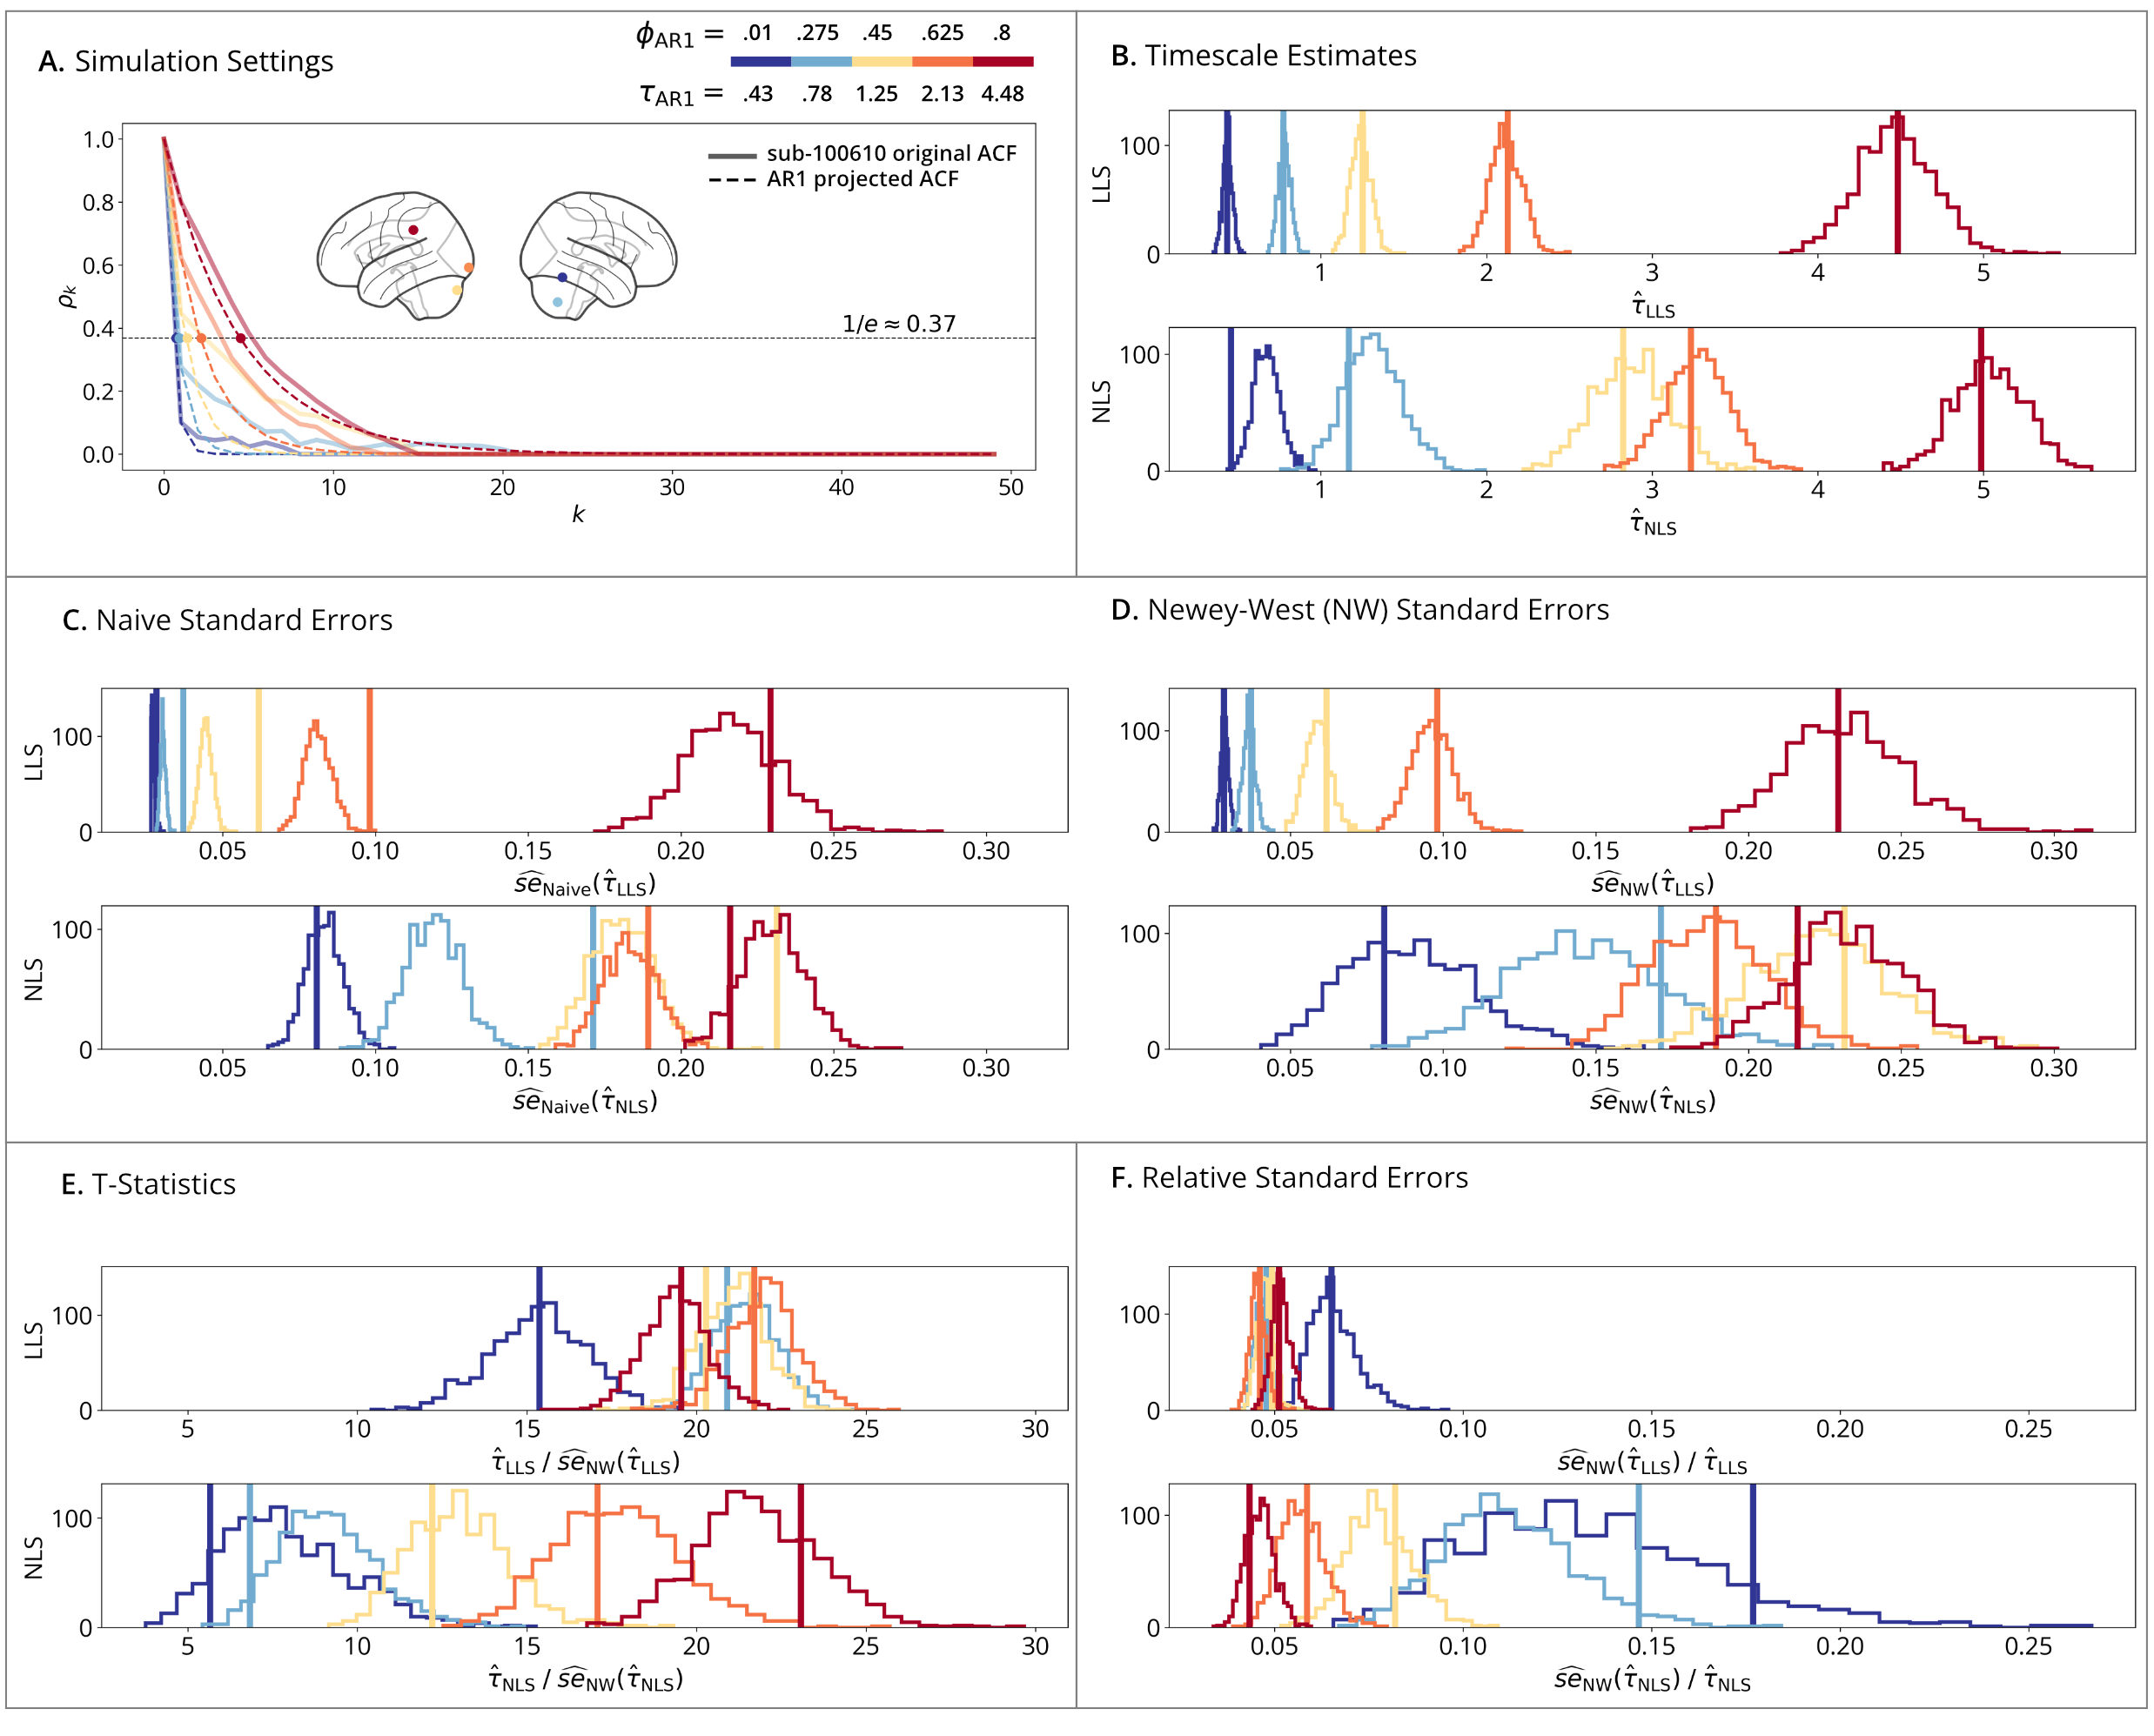
\includegraphics[width=1\textwidth]{latex/results/fig03-hcp.png} 
    \caption{
    \textbf{Human Connectome Project (HCP) simulations}.
    (\textbf{A}) Simulation Settings. Five fixed settings are illustrated, where the solid line represents the original autocorrelation function (ACF) of the specified brain region from subject $\#100610$, and the dashed line represents the AR1-projected ACF. Since the original ACF depends on rfMRI data and the projected is AR1, the lines do not overlap. Solid dots mark the timescale at which the AR1-projected ACF reaches $1/e \approx 0.37$.
    (\textbf{B}) Timescale Estimates. Vertical lines show the true timescale parameters, and histograms show the distribution of timescale estimates across $N=1000$ independent replications. The top plot shows the results for the linear least squares estimator (see \nameref{sec:time-domain-linear-model}), and the bottom plot for the nonlinear least squares estimator (see \nameref{sec:autocorrelation-domain-nonlinear-model}). The true values of the two estimators differ because of their respective definitions.
    (\textbf{C}) Naive Standard Errors and (\textbf{D}) Newey-West Standard Errors. Vertical lines show the standard deviations of the sampling distributions from panel B, while histograms show the distribution of standard error estimates, using the naive and Newey-West estimators, respectively.
    (\textbf{E}) T-Statistics and (\textbf{F}) Relative Standard Errors. Vertical lines show true values, and histograms show the distributions of the estimates.
    }
    \label{fig:sim-hcp}
\end{figure}

\begin{figure}[H]
    \centering
    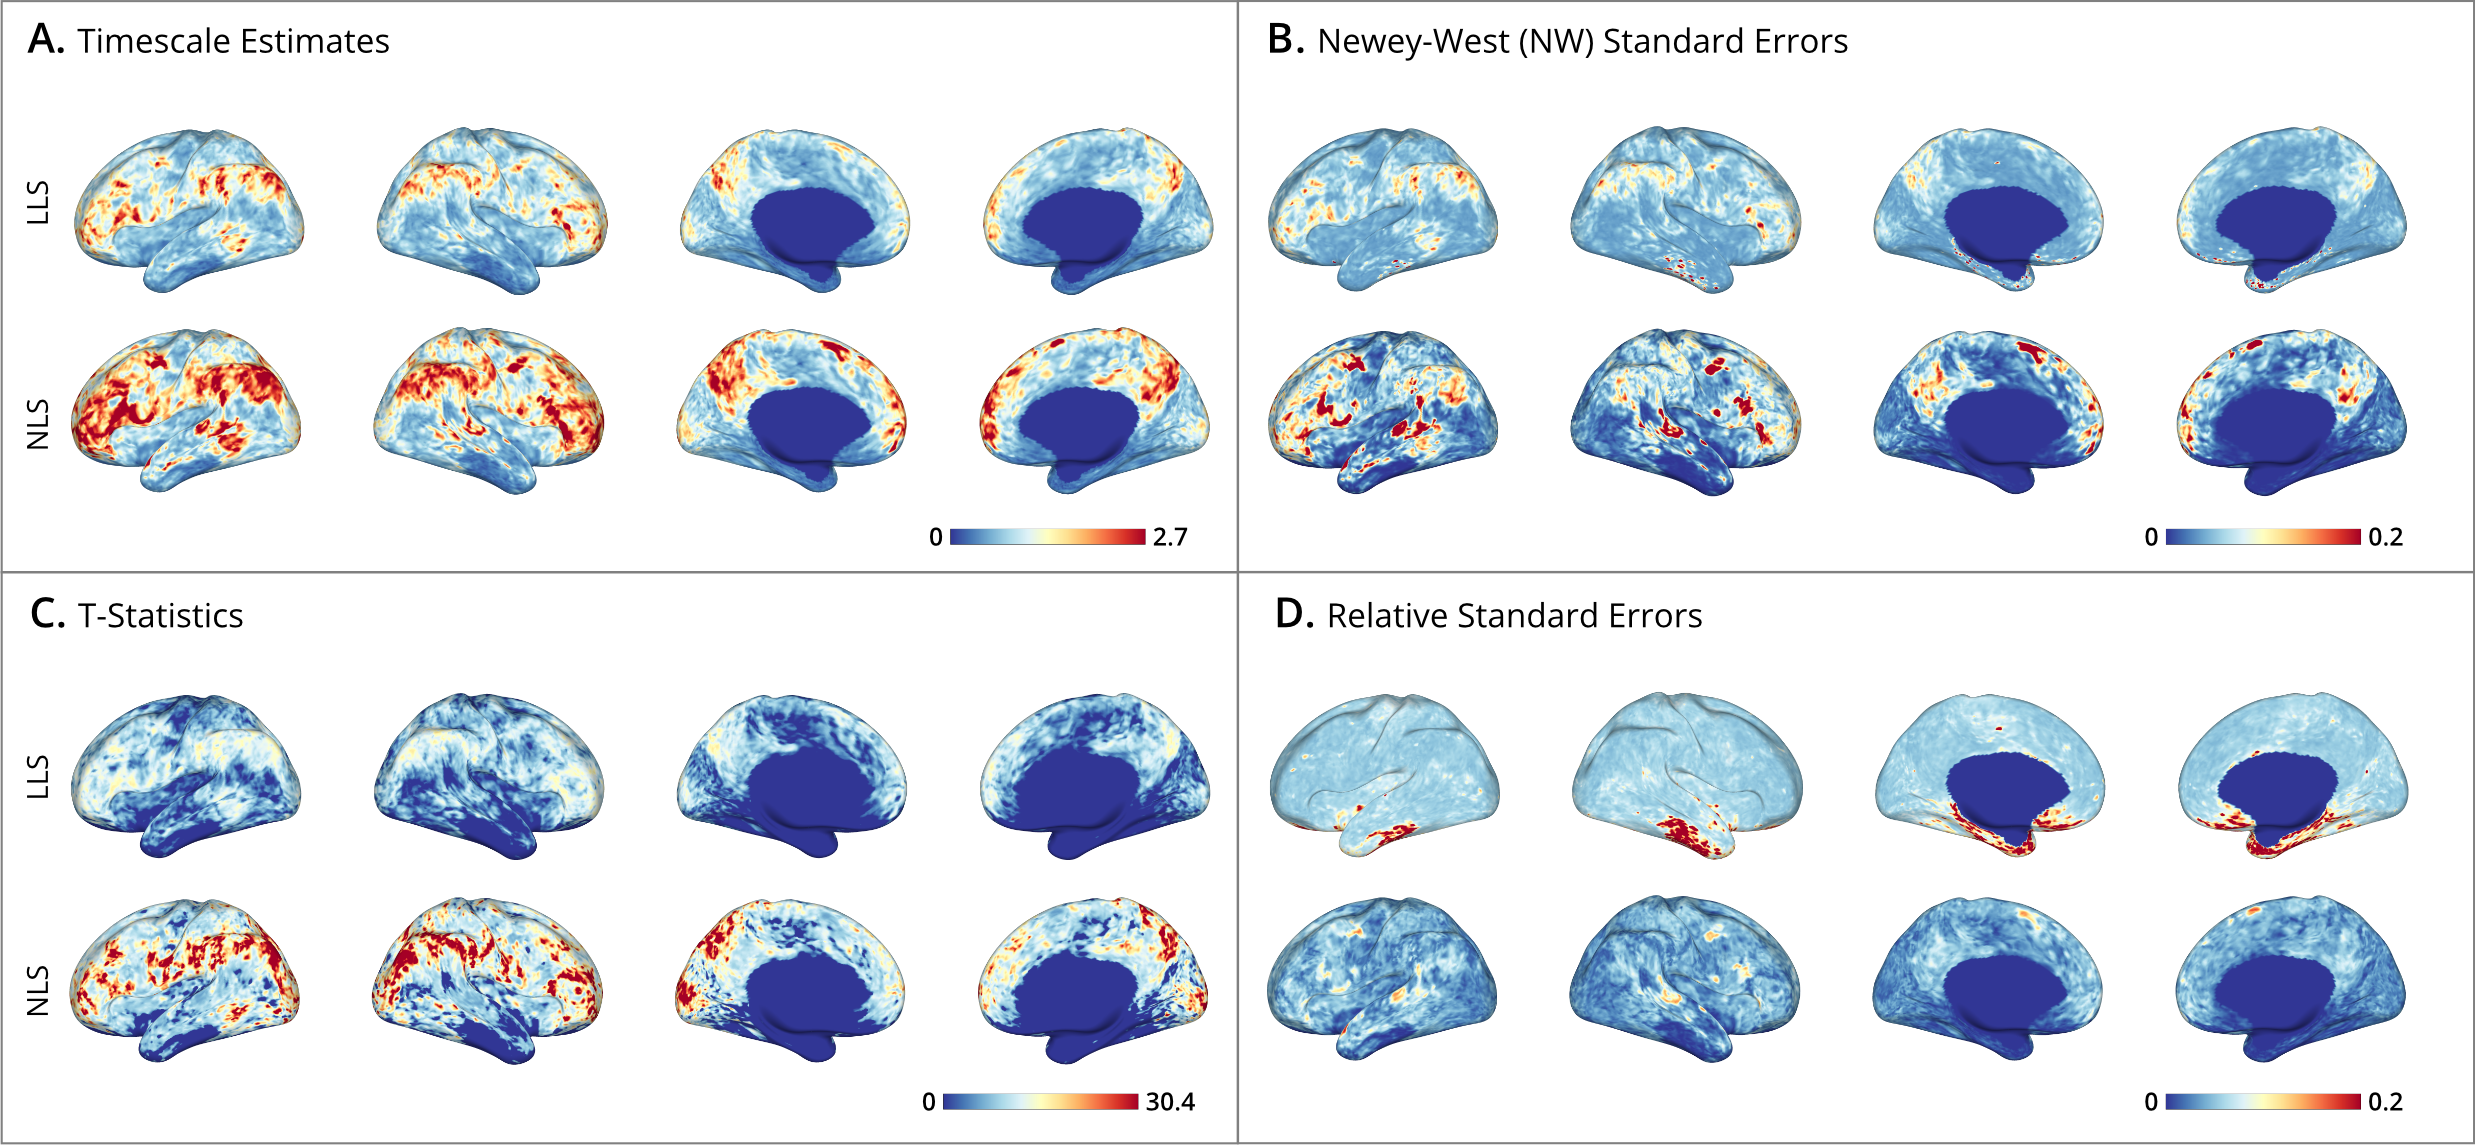
\includegraphics[width=1\textwidth]{latex/results/fig04-hcp1.png} 
    \caption{
    \textbf{Human Connectome Project (HCP) subject-level timescale maps}.
    (\textbf{A-D}) panels display cortical and sub-cortical gray-matter maps from subject $\# 100610$ of the HCP dataset (see \nameref{sec:dataset-description}). The top rows show the results of linear least squares estimator (LLS; see \nameref{sec:time-domain-linear-model}), and the bottom rows show the results of the nonlinear least squares estimator (NLS; see \nameref{sec:autocorrelation-domain-nonlinear-model}). The upper bounds on the colorbars are set for each panel at the $99^\text{th}$ percentile of the cortical map values. 
    }
    \label{fig:map-hcp1}
\end{figure}

\begin{figure}[H]
    \centering
    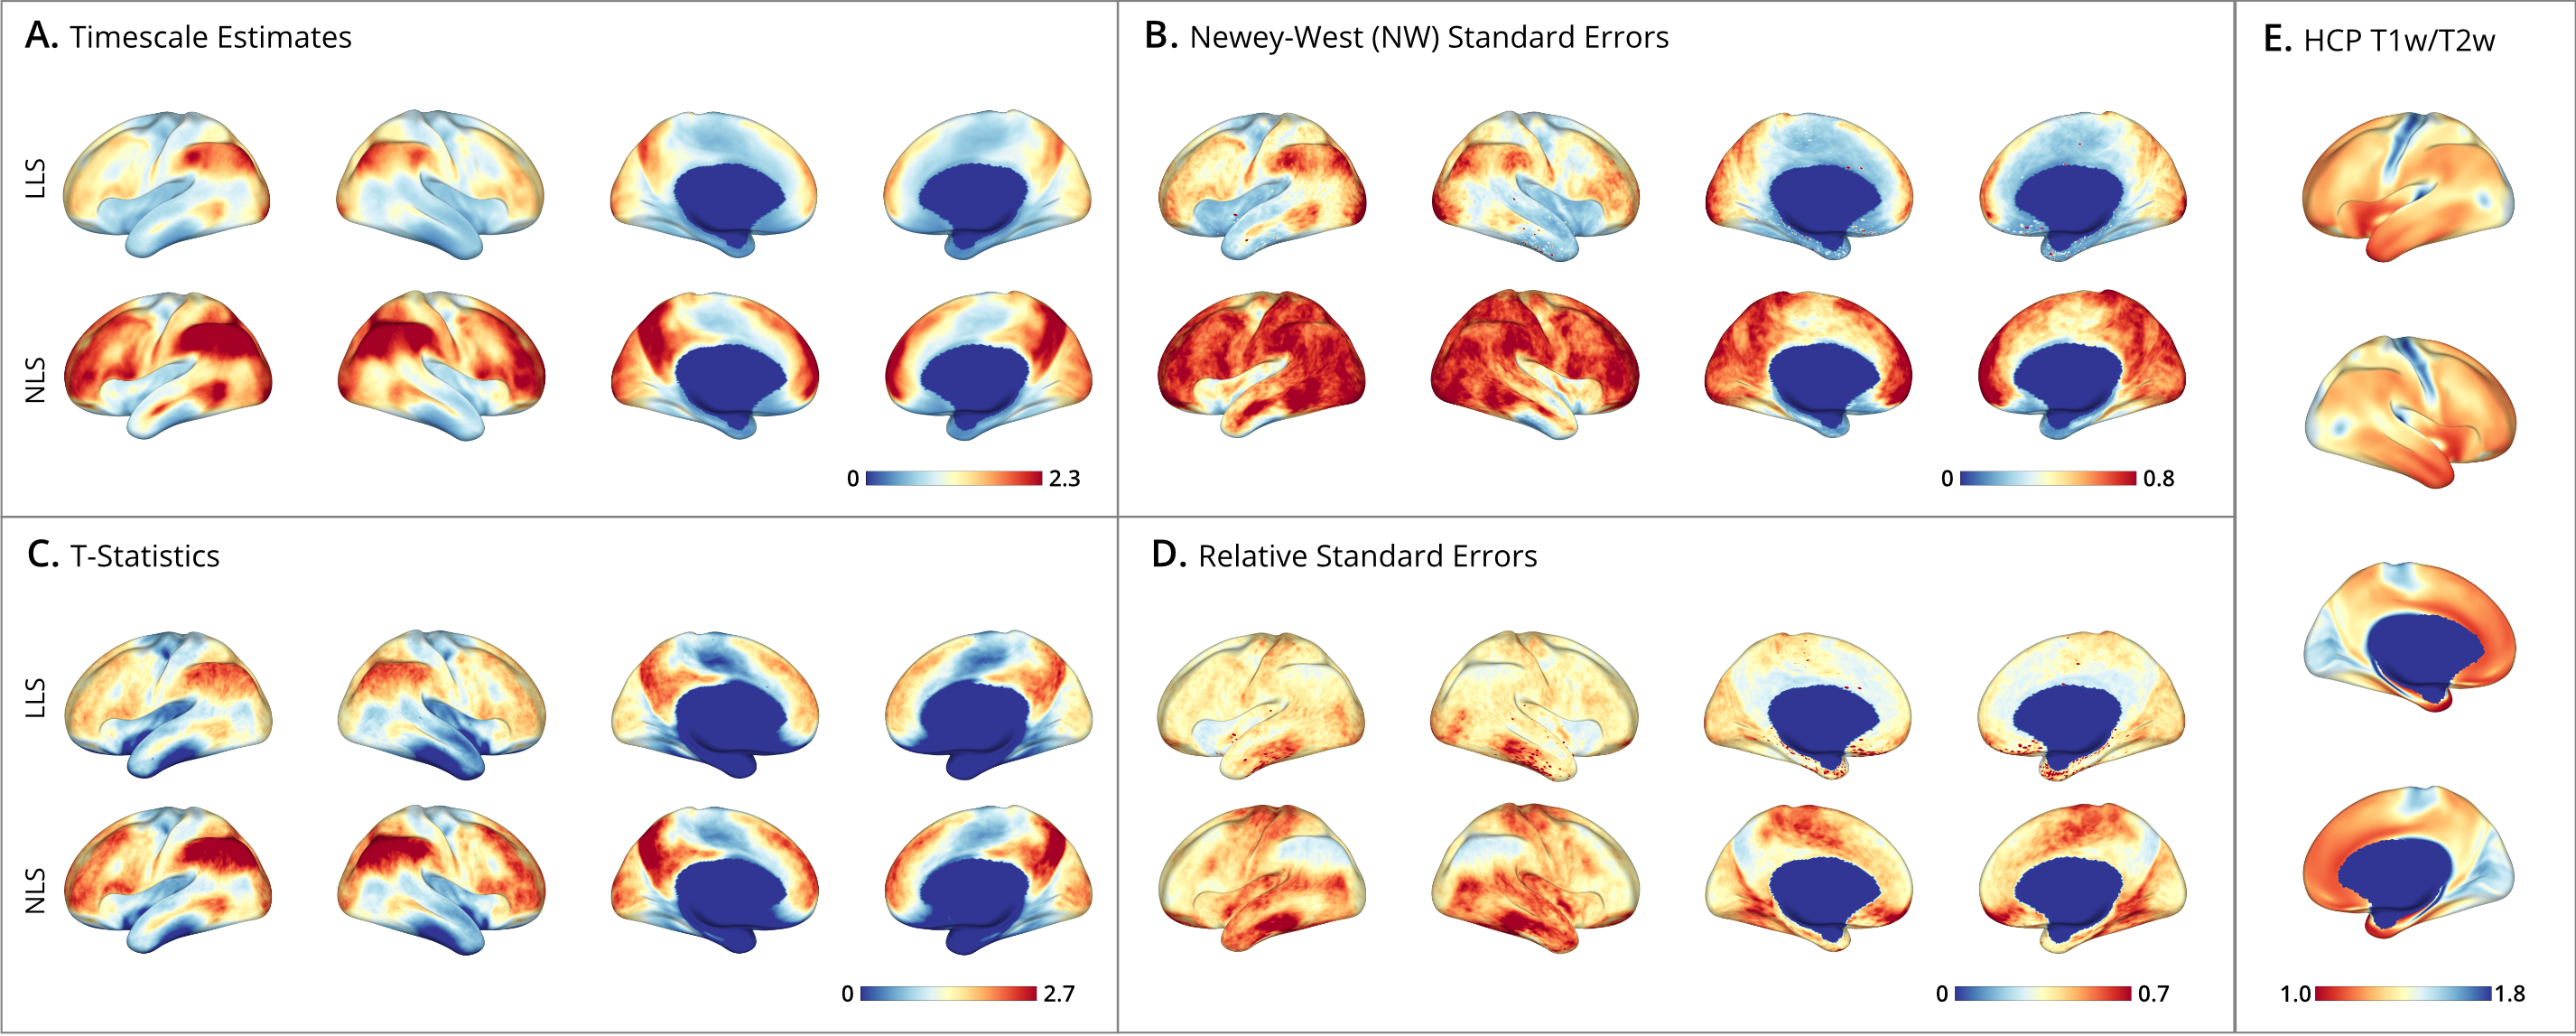
\includegraphics[width=1\textwidth]{latex/results/fig05-hcp180.png} 
    \caption{
    \textbf{Human Connectome Project (HCP) group-level timescale maps.}
    (\textbf{A-D}) panels display cortical and sub-cortical gray-matter maps from $N=180$ subjects of the HCP dataset (see \nameref{sec:dataset-description}). The top rows show the results of linear least squares estimator (LLS; see \nameref{sec:time-domain-linear-model}), and the bottom rows show the results of the nonlinear least squares estimator (NLS; see \nameref{sec:autocorrelation-domain-nonlinear-model}). The upper bounds on the colorbars are set for each panel at the $99^\text{th}$ percentile of the cortical map values. 
    }
    \label{fig:map-hcp180}
\end{figure}
\end{document}


\end{document}